\newgeometry{total={210mm,297mm},left=20mm,right=20mm,bindingoffset=5mm, top=25mm,bottom=25mm} 
\begin{partwithabstract}{Results \& Experiments}
    In this part, the results of different experiments are provided, analysed and interpreted.
    First, experiments were conducted on models training on volume slices along one of the three dimensional axis.
    The performance of these models with respect to their Hyperparameters is analysed.
    Second, the results of different single dimension models are combined to obtain a pseudo mask for training the final model.
    Finally, this model is trained on the pseudo masks.
\end{partwithabstract}
\restoregeometry

\chapter{Single dimension experiments \label{sec:singleDimension}}

\par{
    This chapter discusses the results of several experiments in the construction of single-dimensional models.
    The objective of these experiments is to investigate the influence different model hyperparameters have on the model performance.
    Based on this investigation, the hyperparameters for the single-dimensional models in the final step can be chosen.  
}

\section{Single dimension weakly supervised models}

\par{
    In this section, the results of experiments with different model hyperparameters are compared to each other.
    The point annotation sets are generated from the available full annotation masks for each individual slice.
    In this work, different datasets were used with different levels of provided annotation. 
    Annotation differences between different datasets are listed in table \ref{tab:datasetReferences} on page \pageref{tab:datasetReferences}.
}
\par{
    For three datasets\footnote{The 3 datasets for which full annotation is available are the xVertSeg dataset, the UniSiegen dataset and the MyoSegmentum dataset. Of which the MyoSegmentum dataset is the largest by far.},
    full annotation masks are available, meaning that these scan volumes are labelled with volumes for each the the five lumbar vertebrae.
    For each voxel, the ground truth is indicated up to the point of knowing wether it belongs to a lumbar vertebra and if so, which vertebra.
    For one dataset (PLoS) only semantic segmentation is available. This means that the lumbar vertebrae are indicated, but not destinguished. 
    With each voxel in the PLoS dataset, a ground truth is associated that indicates if it belongs to a lumbar vertebra. There is no label however to indicate which of the lumbar vertebrae this is.
}
\par{
    When a scan is sliced along the craniocaudal axis\footnote{
        The nomenclature of anatomical planes and axis is illustrated in figure \ref{fig:anatomicalPlains} on page \pageref{fig:anatomicalPlains}.
        The craniocaudal axis is the vertical axis when the patient is standing up.} 
    a human can distinguish all 5 lumbar vertebrae (after some practice).
    One may therefor hope the single-dimension models trained on sagittal or frontal slices will be able to do the same.
    Eventhough delineation of a vertebra on a transverse slice is possible. 
    Yet, identification of which vertebra is presented is a very difficult task for a human.
    Supported by a brief test, it was confirmed that trying to estimate 5 vertebra classes from the transverse slices only provides very confused results.
    The models trained on the transverse slices only intend to label the slice pixels as either background (0) or vertebra (1), 
    whereas the models trained on the sagittal and frontal slices intend to indicate which of 6 classes\footnote{0 for background, 1 for $L1$, 2 for $L2$, 3 for $L3$, 4 for $L4$ and 5 for $L2$} the pixel belongs to.
}
\par{
    The models trained to segment sagittal and frontal slices were trained on datasets xVertSeg, UniSiegen and MyoSegmenTUM.
    From the available full masks, point annotation labels were extracted.
    The models trained to segment transverse slices\footnote{This segmentation is, as stated not based on destinguising separate lumbar vertebrae from each other.} 
    are trained on the same three datasets and additionally on the PLoS dataset.    
}
\par{
    Comparison of the model performance results is made based on the weighted dice score calculated on the test set.
    This metric is described in chapter \ref{sec:dice} on page \pageref{sec:dice}.
}


\subsection{Evaluation of the model Hyperparameters}

\par{
    With the objective to obtain the best model hyperparameters to train the single-dimension models, several tests were conducted to estimate the influence of model components and model hyperparameters\footnote{
        One could argue that the number of annotation points is not a \textit{model} hyperparameter. It is an important parameter for the \textit{modelling} approach in general.
    } on the model performance.
}

\subsubsection{Weighted vs. unweighted point loss performance}

\par{
    Equation \ref{eq:LP} on page \pageref{eq:LP} defines the point loss $\mathcal{L}_P$. 
    In this equation, the factor $w_{\mathcal{Y}_i(\vec{p})}$ indicates a weight that can be assigned to each of the output classes.
    Since data classes can be unbalanced, these weights can help to counter this imbalance.
    In this problem (based on the available datasets) there are about 500 times more background voxels than voxels belonging to a lumbar vertebra.
    By weighing with a factor proportional\footnote{The weighting vector is normalized.} to this ratio, this imbalance can be countered\footnote{
        When full data labels are available the counts of the voxel types are available for the train set (one should not include the counts of the validation \& test set to avoid data leakage).
        In principle, this information is not necessarily available when only point level annotation is available. In this work, it is considered that (at least an approximation) of the ratios can be available as prior knowledge.
    }. In the unweighted case, $w_{\cdot} = 1$.
}
\par{
    In figure \ref{fig:weighted_vs_unweighted}, the difference between the weighted dice score \& the average dice score on the test set is compared for two models trained on the transverse slices.
    This result shows the result of the non-weighted segmentation is better than the result of the model trained with weighted loss.
    Contrary to fully supervised models, in the weakly supervised case, the ratio between \textit{labelled} points is not as unbalanced as the ratio between the actual class pixels in the result.
    This explains the weighted point loss performance compared to the unweighted point loss performance.
    An approach that is not tested in this work is to weigh proportional to the inverse of the number of \textit{annotation} points per class instead of weighing proportional to the number of \textit{ground truth} pixels.
}


\begin{SCfigure}[][htb]
    \centering
    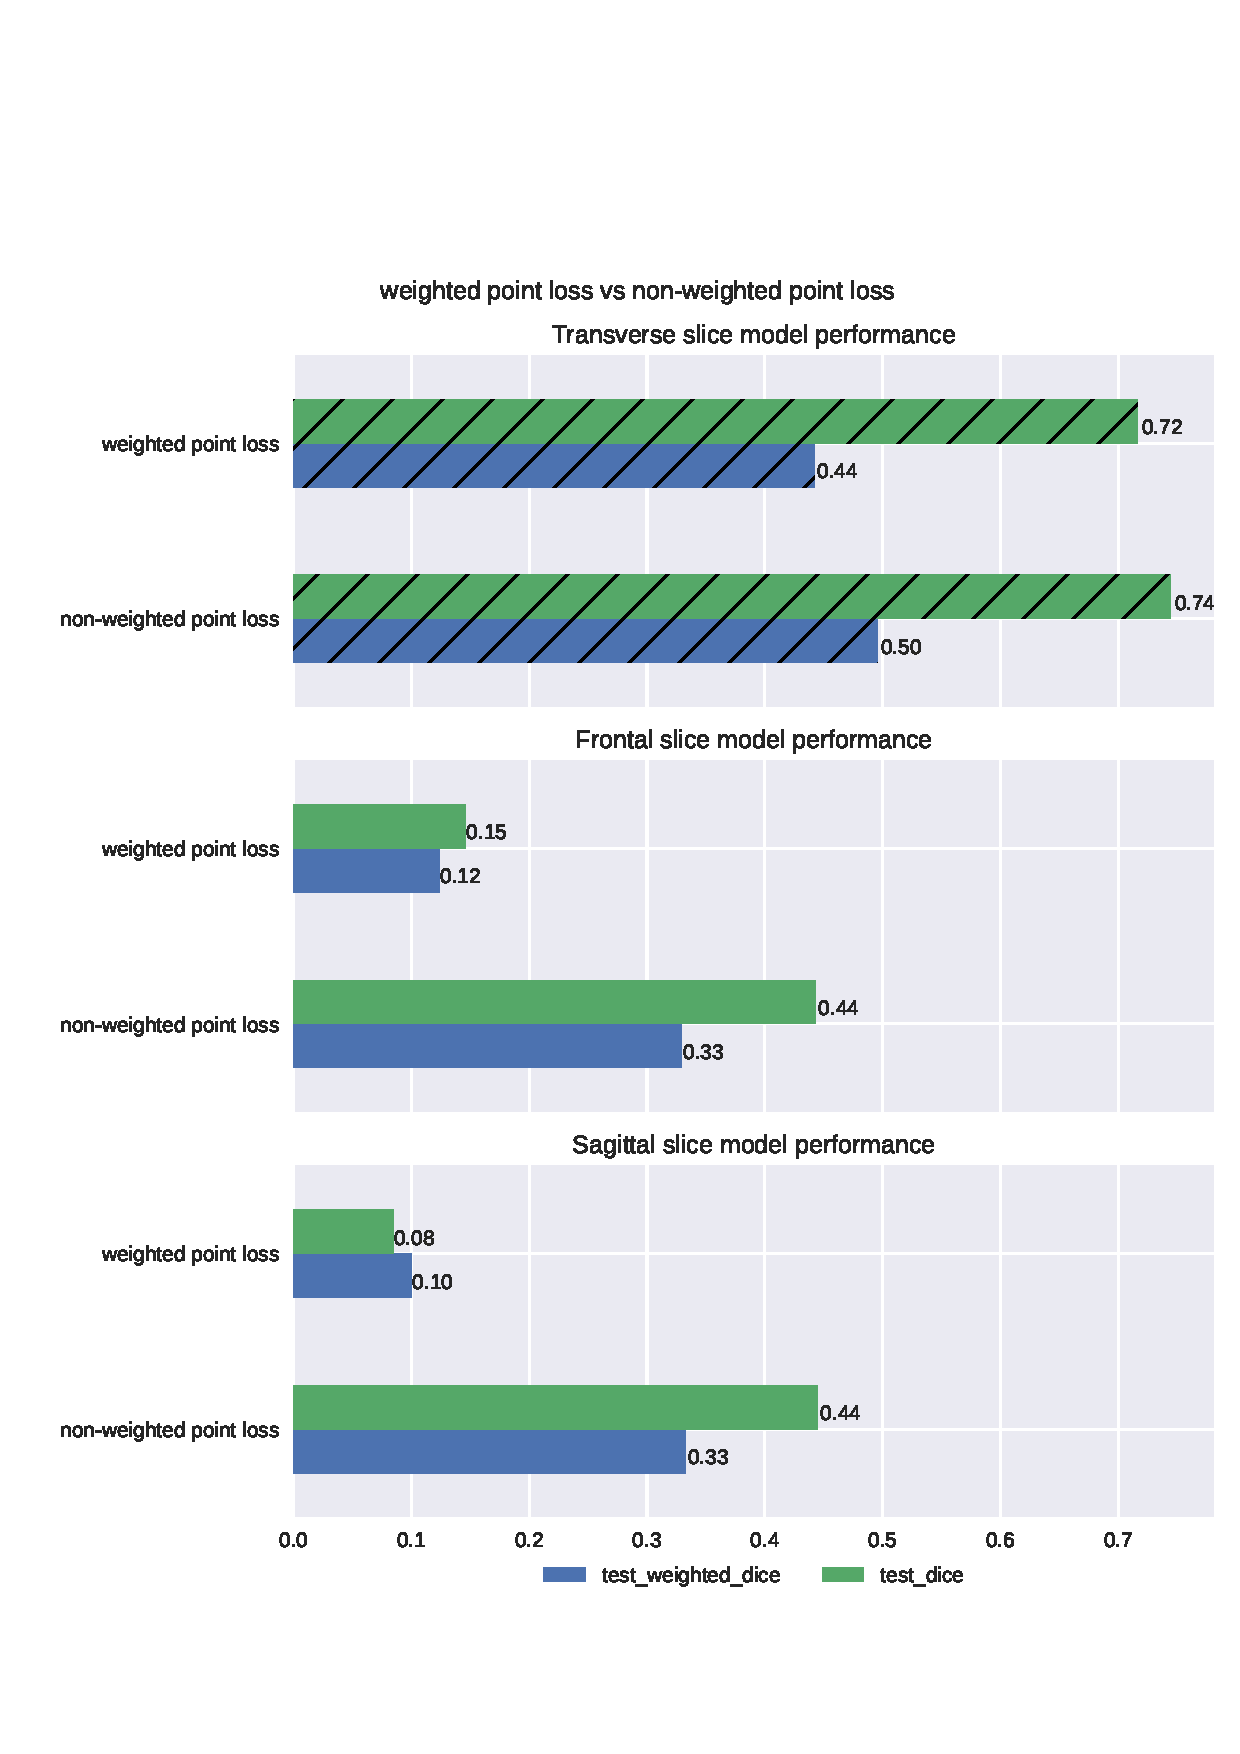
\includegraphics[width=.95\textwidth]{images/weightedvsnonweighted.png}
    \caption{Illustration of the difference in model performance between a weighted point loss function and the unweighted point loss function\label{fig:weighted_vs_unweighted}}
\end{SCfigure}

\subsubsection{Value of the added loss components}
\par{
    In this work, two loss components were added to the consistency loss published in \cite{Laradji}.
    The four loss components used in this work are described in more detail in \ref{sec:LossFunctions}.
    Where \cite{Laradji} is based only on the point loss $\mathcal{L}_P$ and the consistency loss $\mathcal{L}_C$, this work makes use of two extra loss components:
    the prior extend loss $\mathcal{L}_E$ and the separation loss $\mathcal{L}_S$.
    Figure \ref{fig:addedLossComponents} shows experimental results validating the positive influence these added loss terms have on the model performance.
}


\begin{SCfigure}[][htb]
    \centering
    \includegraphics[width=.95\textwidth]{images/TransverseModel_Losscomponents.png}
    \caption{Evaluation of the added value of loss components. \label{fig:addedLossComponents}}
\end{SCfigure}

\subsection{Evolution of the model performance with increased labelling effort}
\par{
    Probably the most basic modelling hyperparameter for a point annotation modelling campaign is the number of labelling points one asks the expert to provide.
    This section presents experimental results to estimate the influence of the number of annotation points on the resulting model performance.
    Intuitively, one would expect the model performance increases with the number of annotation points provided.
    This turns out to be false.
}


\chapter{Single dimension model combination\label{sec:combination}}
In chapter \ref{sec:singleDimension}, the construction of single dimension models is discussed.
These models extimate the segmentation masks of $352\times 352$ patches of scan volume slices along one of the three main axis.
In this chapter, the results of these single dimension models are combined to form a \textit{pseudo} mask that is subsequently used as labelling to train the final segmentation network.
Interesting to note in this procedure is that the evaluation metric of these obtained segmentation masks is improved in each of these steps.
The pseudo mask volume performs better than the single dimension model results and the final model trained on the pseudo masks performs better than the pseudo mask itself. 

\section{Volume combination procedure}
To construct one pseudo mask volume, first, three single dimension model are evaluated to form three stacks of two dimensional estimated segmentation masks, which are then combined to form three segmentation volumes. 
The resulting set of three segmentation volumes is then combined to form a new segmentation volume.
It is this last segmentation volume, made out of the combination, that is sliced again to obtain the pseudo masks for the final model.

\subsection{Recombination of the crops to slices}
All models are designed for $352 \times 352$ crops of the 2D slices\footnote{More information on the cropping of the slices can be found in chapter \ref{sec:cropping} on page \pageref{sec:cropping}.}.
To construct a segmentation volume from a single dimensional model, all relevant\footnote{Some slices have dimensions that do not allow to extract 5 different $352 \times 352$ crops. See for example figure \ref{fig:smallcrop} on page \pageref{fig:smallcrop}.} crops of each volume slice are evaluated.
First the segmentation results on these crops have to be combined again to obtain a segmentation mask of the whole slice.
Due to the cropping procedure, different crops of the same slice always partly overlap.
The crops are combined by averaging the logits $z_i$ for the overlapping positions.
The inferred class is then obtained from the resulting average $z_i$ values for that position. 

\subsection{Rule based result combination}
Once a stack of class segmentation masks for all slices of a volume are obtained, these can be combined to form a segmentation volumes.
Combining the results of three different single dimension models is performed in two steps:
\begin{enumerate}
    \item The resulting classification volumes are first combined with a rule-based method.
    \item After this rule-based combination, the resulting segmentation estimation is smoothened with a morphological filter.
\end{enumerate}

Three single dimension models are trained:
\begin{description}
    \item[Transverse slices] offer little context to indicate which of the lumbar vertebrae they contain. 
    It does not seem easy even for a human expert to indicate which vertebra is visible on the slice.
    The model trained on these slices is intended only for semantic segmentation.
    Each pixel is inferred only if it represents a vertebra, without distinction between the different lumbar vertebrae. 
    \item[Sagittal \& Coronal slices] do offer the necessary context to distinguish between $L_1$ to $L_5$. 
    The models trained on these slices do indicate the specific lumbar vertebra index. 
\end{description}

The volume combination rules are based on two observations:\footnote{
    The resulting estimations from a model for an input volume is again a three-dimensional volume ($\in \mathbb{N}^3$) with the same dimensions.
}.
\begin{enumerate}
    \item The precision (see equation \ref{eq:precision_i} on page \pageref{eq:precision_i}) with which the background class is predicted in all models is very high.
            This means $\mathcal{P} \left( label = background \mid prediction = background \right)$ is high for all models. 
            If there is one model that indicates a position is background, this position could be estimated to be background with high probability.
    \item The rule mentioned above can be nuanced\footnote{The opportunity to use the results of the other two single dimension models to correct a \textit{lapse} of one of the single dimension models can be recognized as one of the strengths of the combination procedure.}.
    It was observed that single dimension models can miss the mask\footnote{This is caused by the large differences between the different datasets used, see chapter \ref{sec:datasets} at page \pageref{sec:datasets}.}. 
    For some volumes, the recall of the vertebra class is extremely low. The single dimension model predicts the background class for allmost all positions.
    When this is observed, it does not make much sense to stick to the first rule.
\end{enumerate}
The observations mentioned above can be combined in algorithm \ref{alg:combination}.

\subsection{Morphological smoothing}
After the rule-based combination of estimations from different single dimension models, the result is smoothened with standard morphological filters.
These filters are combinations of the morphological \textit{erosion} and \textit{dilation} operators\footnote{
    This document is not intended to provide an elaborate explanation on morphological operations.
    For the readers conventience, the following symbolic notations are repeated:
    \begin{description}
        \item[Erosion] of set $\mathbf{A}$ by structural element $\mathbf{B}$ : $\mathbf{A} \ominus \mathbf{B}$ 
        \item[Dilation] of set $\mathbf{A}$ by structural element $\mathbf{B}$ : $\mathbf{A} \oplus \mathbf{B}$ 
        \item[Opening] of set $\mathbf{A}$ by structural element $\mathbf{B}$ : $\mathbf{A} \circ \mathbf{B} = (\mathbf{A} \ominus \mathbf{B}) \oplus \mathbf{B}$
        \item[Closing] of set $\mathbf{A}$ by structural element $\mathbf{B}$ : $\mathbf{A} \bullet \mathbf{B} = (\mathbf{A} \oplus \mathbf{B}) \ominus \mathbf{B}$
    \end{description}
}.

\begin{itemize}
    \item Noise in the single dimension segmentation masks is suppressed with an opening operation on the individual segmentation volumes of the single dimension models.
    \item Noise in the combined volumes is suppressed by first opening and then closing the volumes.
    \item The estimated volumes are observed to overestimate the extent of the vertebrae. For this reason, an erosion step is performed to decrease the overall extent of the class masks.
\end{itemize}

The procedure mentioned above has two hyperparameters: the number of iterations for the denoising filters and the number of iterations for the erosion filter.
Both hyperparameters are estimated by calculating the same evaluation metric, the weighted dice score on the validation set, as for the single-dimensional model evaluation. 

\subsection{Volume combination algorithm}
The combination of the rules and morphological smoothing operations discussed above result in the following algorithm to combine the segmentation volumes from the single dimension models\footnote{
    The cardinality of a set $\mathbf{A}$, written as $|\mathbf{A}|$, is the number of elements in a set.
    The cardinality of the class label sets $c_.$ thus represents the voxel count in each segmentation volumes that is estimated to be \textit{not background}.
    Suspiciously low voxel counts classified other than background are defined as lower than 35\% of the highest class label cardinality.
    This last factor has not been optimised. It is an engineering estimate.
    If a volume is found to be have such a low class label cardinality, this volume reference is stored as $d_{ignore}$ and the volume is ignore in the combination protocol.
    In practice, the low cardinality volumes are all the segmentation volumes obtained from the model trained on point annotated tranverse slices.
}:

\begin{algorithm}[H]
    \SetAlgoLined
    \KwData{
        Results $y_.$ of three models indicating an estimated class for all positions $\vec{p}$ in the volume. \;
        Transverse model $y_t \in \mathbb{N}^3: \forall y_t(\vec{p}) \in \{ 0, 1 \}$ \;
        Sagittal model $y_s \in \mathbb{N}^3: \forall y_t(\vec{p}) \in \{ 0, 1, 2, 3, 4, 5 \}$ \;
        Coronal model $y_c \in \mathbb{N}^3: \forall y_t(\vec{p}) \in \{ 0, 1, 2, 3, 4, 5 \}$  \;
        Binary $\mathbf{B}$ structure with rank 3 and connectivity 3 \;
    }
    \KwResult{Combination of the three model results $y_f$.}
    \tcp{Closing operation on all $y_.$}
    $y_t \leftarrow y_t \bullet \mathbf{B}$ \;
    $y_s \leftarrow y_s \bullet \mathbf{B}$ \;
    $y_c \leftarrow y_c \bullet \mathbf{B}$ \;
    \tcp{(relative) cardinality of the class label sets}
    $c_t \leftarrow |\{ y_t \neq 0 \}|$ \;
    $c_s \leftarrow |\{ y_s \neq 0 \}|$ \;
    $c_c \leftarrow |\{ y_c \neq 0 \}|$ \;
    $r_t \leftarrow \frac{c_t}{max(c_t, c_s, c_c)}$ \;
    $r_s \leftarrow \frac{c_s}{max(c_t, c_s, c_c)}$ \;
    $r_c \leftarrow \frac{c_c}{max(c_t, c_s, c_c)}$ \;
    \lIf{$\exists d \in [ t,s,c ] : r_d < 0.35$}{$d_{ignore} \leftarrow d$}\lElse{$d_{ignore} \leftarrow \emptyset$}
    \For{all $\vec{p}$}{
        $i \in [ 1, 2, 3, 4, 5]$ \;
        \Switch{$d_{ignore}$}{
            \Case{$\emptyset$}{
                \lIf{$y_t[\vec{p}] = 1 \wedge y_s[\vec{p}] = i \wedge y_c[\vec{p}] = i$}{
                    $y_f[\vec{p}] \leftarrow i$ 
                }
                \lElse{
                    $y_f[\vec{p}] \leftarrow 0$ 
                }
            }
            \Case{$t$}{
                \lIf{$y_s[\vec{p}] = i \wedge y_c[\vec{p}] = i$}{
                    $y_f[\vec{p}] \leftarrow i$ 
                }
                \lElse{
                    $y_f[\vec{p}] \leftarrow 0$
                }
            }
            \Case{$s$}{
                \lIf{$y_t[\vec{p}] = 1 \wedge y_c[\vec{p}] = i$}{
                    $y_f[\vec{p}] \leftarrow i$ 
                }
                \lElse{
                    $y_f[\vec{p}] \leftarrow 0$ 
                }
            }
            \Case{$c$}{
                \lIf{$y_t[\vec{p}] = 1 \wedge y_s[\vec{p}] = i$}{
                    $y_f[\vec{p}] \leftarrow i$ 
                }
                \lElse{
                    $y_f[\vec{p}] \leftarrow 0$ 
                }
            }
        }
    }
    $y_f \leftarrow ((y_f \circ \mathbf{B}) \bullet \mathbf{B}) \ominus \mathbf{B}$
   \caption{Rule based combination of model results from three single dimension models\label{alg:combination}}
\end{algorithm}

\section{Pseudo mask performance}
Using algorithm \ref{alg:combination}, a segmentation volume can be obtained with a higher weighted dice metric than the each of the individual segmentation volumes obtained from the single dimension models.
This is tested by combining three models.
Table \ref{tab:combination_1} illustrates this concept.

\begin{SCtable}[\sidecaptionrelwidth][h]

    \begin{tabular}{l|lll}
        \hline
        \textbf{\begin{tabular}[c]{@{}l@{}}Slice \\ direction\end{tabular}} &
          \textbf{Transverse} &
          \textbf{Coronal} &
          \textbf{Sagittal} \\ \hline
        \begin{tabular}[c]{@{}l@{}}Context\\ Slices {[}mm{]}\end{tabular}   & 1     & 1     & 1     \\ \cline{1-1}
        \begin{tabular}[c]{@{}l@{}}Points per\\ class instance\end{tabular} & 1     & 1     & 1     \\ \cline{1-1}
        \begin{tabular}[c]{@{}l@{}}Background \\ points\end{tabular}        & 5     & 3     & 3     \\ \cline{1-1}
        Dataset &
          \begin{tabular}[c]{@{}l@{}}PLoS\\ xVertSeg\\ USiegen\\ MyoSegmenTUM\end{tabular} &
          \multicolumn{2}{l}{\begin{tabular}[c]{@{}l@{}}xVertSeg\\ USiegen\\ MyoSegmenTUM\end{tabular}} \\ \cline{1-1}
        \begin{tabular}[c]{@{}l@{}}Segmentation\\ classes\end{tabular}      & 2     & 6     & 6     \\ \cline{1-1}
        \begin{tabular}[c]{@{}l@{}}Weighted \\ dice score\end{tabular}      & 0.476 & 0.339 & 0.350 \\ \hline
        \begin{tabular}[c]{@{}l@{}}Weighted\\ dice score\\ combination\end{tabular} &
          \multicolumn{3}{c}{\textit{0.51}} \\ \hline
        \end{tabular}
    \caption{Combination of three point supervised models with algorithm \ref{alg:combination}. 
    These models were constructed with a fixed number of background points and a fixed number of class labels per class instance.
    This test indicates that the segmentation mask obtained from the result of single dimension models with algorithm \ref{alg:combination} allows to obtain a new segmentation mask with a higher metric score, the pseudo masks.
    Pay attention, the weighted dice scores for the individual models are evaluated on the test set, while the weighted dice score for the combination is evaluated on the cross validation set. \label{tab:combination_1}
    }

\end{SCtable}

In table \ref{combination_1}, the segmentation quality is calculated on the validation set.
Since there are two hyperparameters (the number of denoise iterations and the number of erosion iterations) to optimise in the combination algorithm \ref{alg:combination}, 
the algorithm is evaluated with a matrix of these hyperparameters and 

\marginpar{
        \includegraphics{images/combination_optimization_1.png}
        \captionof{figure}{Illustration of the hyperparameter optimization procedure for the combination detailed in \ref{combination_1}}
        \label{fig:hyperparameter_combination_1}
    }

\begin{SCfigure}[][htb]
    \centering
    \includegraphics[width=.95\textwidth]{images/morphmask_denoise1_erode1_MyoSegmenTUM_036.png}
    \caption{
        Result of the combination of the three single dimension model results for volume MyoSegmenTUM nr 43.
        The colours indicate the vertebra classes. Only one semantic class is estimated in the first row, illustrating the model trained on transversal slices.
        On the first three rows, slices of the resulting segmentations from the single dimension models are shown. 
        It is clear these masks contain some artefacts and are not always in agreement with each other.
        On the fourth row, the result after mask combination and morphological smoothing is shown. 
        This corresponds more closely to the ground truth mask, shown on the fifth row.
        This final mask, shown on the fourth row, will be used as a pseudo mask to approximate the unknown ground truth mask.
        In the last row, the corresponding images are shown.
    }
\end{SCfigure}

\chapter{Pseudo mask training}

Time to evaluate
performance